\documentclass[hyperref={unicode=true}]{beamer}

\usepackage[utf8]{inputenc}
\usepackage[english,russian]{babel}
\usepackage{../clrscode3e} 
\usepackage{xcolor}
\usepackage{pstricks, pst-tree, pst-node}
\usepackage{graphics}

%\usepackage{beamerthemesplit}

\AtBeginSubsection[]
{
  \begin{frame}<beamer>{Раздел}
    \tableofcontents[currentsection,currentsubsection]
  \end{frame}
}

\newtheorem{rtheorem}{Теорема}
\title{Цифровой поиск}
\subtitle{Дискретный анализ 2012/13}
\author{Андрей Калинин, Татьяна Романова}
\date{1 октября 2012\,г. }
\usetheme{default}
\usefonttheme[onlymath]{serif}


\begin{document}
\psset{levelsep=1cm, treesep=1cm, linewidth=0.5pt, levelsep=30pt}
\newcommand{\tnd}[1]{\Tcircle{\makebox[5mm][c]{#1}}}
\newcommand{\nilnd} {\Tp[edge=none]}
\newcommand{\rednd}[1]{\Tcircle[linecolor=red!30, %
    fillstyle=solid, fillcolor=red!30] {\makebox[5mm][c]{#1}}}
\newcommand{\blacknd}[1]{\Tcircle[linecolor=black!20, %
    fillstyle=solid, fillcolor=black!20]{\makebox[5mm][c]{#1}}}

\frame {\titlepage}

\frame
{ 
\frametitle{Литература}
  \begin{itemize}
    \item Д. Э. Кнут, Искусство программирования, том 3, п. 6.3 Цифровой поиск, с.\,527-535.
  \end{itemize}
}

\section{Цифровой поиск}
\subsection{Дерево ключей}

\frame
{
  \frametitle{Способ построения}
  \begin{itemize}
    \item Цифровой поиск основан не на сравнении ключей, а на их представлении в виде последовательности букв или цифр.
    \item Пример --- побуквенные метки в больших словарях.
    \item Простейшая реализация --- дерево ключей. Пусть $M$ --- мощность алфавита, $N$ --- количество ключей. В каждом узле может храниться массив указателей размером $M$ или, если $M$ велико, а $N$ нет, линейный список.
    \item Ни один ключ, хранящийся в дереве, не является префиксом другого.
  \end{itemize}
}

\frame
{
  \frametitle{Пример}
  Дерево ключей со словами this, that, car, care, cat:\\
~\\
~\\
  \begin{figure}[h!]
  \centerline{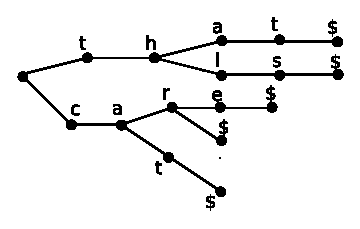
\includegraphics{keytree.eps}}
  \end{figure}
}

\frame
{
  \frametitle{Недостатки}
  \begin{itemize}
    \item Нерациональный расход памяти.
    \item Считывание из памяти строки при каждом обращении к узлу.
    \item Невозможность хранить строки на диске из-за большого количества чтений при поиске.
  \end{itemize}
}

\section{PATRICIA}
\subsection{Структура дерева}
\frame
{
  \frametitle{Основные идеи}
  \begin{itemize}
    \item Practical Algorithm to Retrieve Information Coded in
      Alphanumeric. 
    \item Используется бинарный алфавит.
    \item Во внутреннем узле хранится количество битов, которые можно
      пропустить до проверки очередного бита. Эти биты общие для всех
      потомков. 
    \item Дерево не содержит однопутевых веток.
    \item Указатель на ключ хранится в листовом узле.
    \item При поиске находится ключ, совпадающий с искомым по
      маске. Затем производится чтение строки (возможно, с диска) и
      сравнение с искомым ключом. 
    \item Все узлы хранятся в памяти, все данные могут храниться на
      диске. 
  \end{itemize}
}

\frame
{
\frametitle{Пример}
Переход от дерева ключей к PATRICIA:\\
~\\
~\\
\begin{figure}[h!]
\centerline{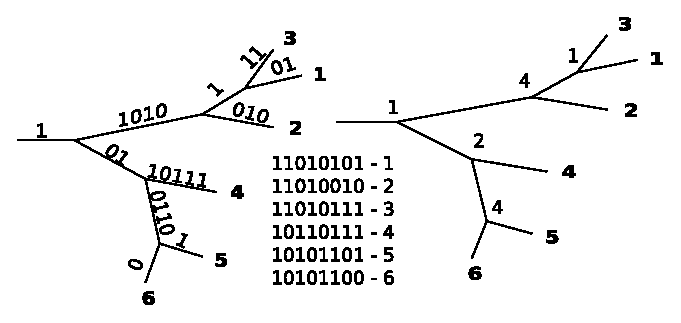
\includegraphics{pat1.eps}}
\end{figure}
}

\frame
{
  \frametitle{Улучшение}
  \begin{itemize}
    \item Количество <<развилок>> (внутренних узлов, считая корень)
      совпадает с количеством листовых узлов. 
    \item Ключи могут храниться вместе с <<развилками>>.
    \item Для указания на хранящийся в листе ключ используется ссылка
      <<вверх>>, помечаемая специальным образом. 
  \end{itemize}
}

\frame
{
\frametitle{Пример}
\begin{figure}[h!]
\centerline{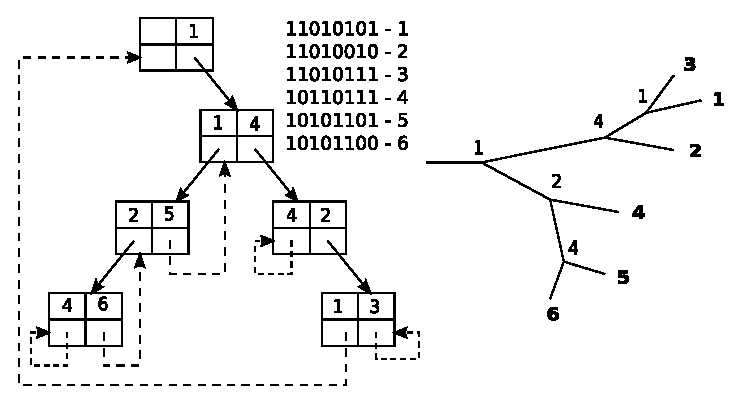
\includegraphics{pat2.eps}}
\end{figure}
}

\frame{
  \frametitle{Структуры данных}
  \begin{itemize}
    \item Ключ:
      \begin{enumerate}
        \item bitlen --- длина ключа в битах. 
        \item data --- массив с данными, можно получить нужный бит
          функцией bit(key,n)
      \end{enumerate}
    \item Узел дерева:
      \begin{enumerate}
        \item key --- номер соответствующего ключа. 
        \item skip --- количество пропускаемых бит. 
        \item links[2] --- ссылки на левое (0) и правое (1) поддерево,
          состоящие из:
          \begin{enumerate}
            \item link --- указателя. 
            \item  up --- признака, что этот указатель ведёт <<наверх>>.
          \end{enumerate}
      \end{enumerate}
  \end{itemize}
}


\subsection{Поиск}

\frame{
\frametitle{Основная идея}
\begin{enumerate}
  \item Проходим по всему дереву, последовательно проверяя нужные
    биты, используя поля skip. 
  \item При проходе по ссылке, помеченной флагом up, считываем из узла
    номер ключа. 
  \item Достаём ключ из базы и сверяем его с искомым: если он равен,
    то мы его нашли, если не равен, то длина совпадающего префикса будет самым
    длинным совпадением из всей базы ключей PATRICIA. 
\end{enumerate}
}

\frame
{
  \frametitle{Алгоритм}
  \begin{codebox}
      \Procname{$\proc{Pat-Search}(T, \id{key})$}
      \li $\id{ref} \gets \&\attribb{T}{root}{links[1]}, \id{pref} \gets \&\attrib{T}{root}$
      \li $\id{nd} \gets \attrib{ref}{link}, j \gets 0$
      \li \While \kw{not} $\attrib{ref}{up}$
          \Do
      \li       $j \gets j + \attrib{nd}{skip}$
      \li       $\id{pref} \gets \id{ref}$
      \li       $\If j < \attrib{key}{bitlen}$ \kw{then} $\id{dir} \gets bit(\id{key},j)$ \kw{else} $\id{dir} \gets 0$
      \li       $\id{ref} \gets \&\attrib{nd}{links[dir]}$
      \li       $\id{nd} \gets \attrib{ref}{link}$
          \End
      \li  $m = \proc{Common-Bit-Prefix}(\attrib{nd}{key}, \id{key})$
      \li \Return $(\id{pref}, \id{dir}, m)$
  \end{codebox}
}

\subsection{Вставка}

\frame{
  \frametitle{Основная идея}
  \begin{enumerate}
    \item Ищем ключ в дереве, вычисляем самый длинный совпадающий
      префикс.
    \item Нужно найти связь, на которую приходится конец этого
      префикса, и разбить её новым внутренним узлом дерева. 
    \item При этом одна из связей нового узла должа будет показывать
      на него самого, а другая --- продолжать старую связь. 
  \end{enumerate}
}

\frame
{
\frametitle{Алгоритм}
  \begin{codebox}
      \Procname{$\proc{Pat-Insert}(T, \id{key})$}
      \li \If $\attrib{T}{empty()}$
          \Then
      \li $\attrib{T}{root} \gets \proc{New-node}(\id{key})$, $\attribb{T}{root}{point-to(1, \attrib{T}{root})}$
      \li \Return $(\const{true}, \attrib{T}{root})$
          \End

      \li $(\id{pref}, \id{dir}, m) \gets \proc{Pat-Search}(T, \id{key})$
      \li \If $m \isequal \attrib{key}{bitlen}$
          \Then
      \li \Return $(\const{false}, \attrib{ref}{link})$
          \End
      \li $\id{ref} \gets \&\attribb{T}{root}{links[1]}, \id{nd} \gets \attrib{ref}{link}, j \gets 0$
      \li \While \kw{not} $\attrib{ref}{up}$ \kw{and} $j + \attrib{nd}{skip} < m$
            \Do
      \li       $j \gets j + \attrib{nd}{skip}$
      \li       $\id{ref} \gets \&\attrib{nd}{links[bit(\id{key}, j)]}$
      \li       $\id{nd} \gets \attrib{ref}{link}$
            \End
      \li  \Return $(\const{true}, \proc{Split-Insert}(\id{ref}, \id{key}, m, m-j))$
  \end{codebox}
}

\frame
{
\frametitle{Алгоритм}
  \begin{codebox}
      \Procname{$\proc{Split-Insert}(\id{ref}, \id{key}, m, k)$}
      \li $N \gets \proc{New-node}(\id{key})$
      \li $\id{dir} \gets bit(key, m)$
      \li $\attrib{N}{point-to(dir, N)}$
      \li $\attrib{N}{links[1 - dir]} \gets *\id{ref}$
      \li $\attrib{N}{skip} \gets k$

      \li \If \kw{not} $\attrib{ref}{up}$
          \Then
      \li $\attribb{ref}{link}{skip} \gets \attribb{ref}{link}{skip} - k$
          \End
      \li $\attrib{ref}{link} \gets N$
      \li $\attrib{ref}{up} \gets \const{false}$
      \li \Return $N$
  \end{codebox}
}

\subsection{Удаление}

\frame{
  \frametitle{Основная идея}
  \begin{itemize}
    \item В худшем случае нужно модифицировать два узла: узел со
      ссылкой <<вверх>> и узел, где хранится номер удаляемого ключа. 
    \item Выполняем удаление в два этапа:
      \begin{enumerate}
        \item Перемещаем ключ из листа в узел, где содержится
          удаляемый ключ, тем самым ссылка <<вверх>> будет вести на
          тот же узел.
        \item После чего удаляем лист.
      \end{enumerate}
  \end{itemize}
}

\frame
{
\frametitle{Алгоритм}
  \begin{codebox}
      \Procname{$\proc{Pat-Delete}(T, \id{key})$}
      \li $(\id{pref}, \id{dir}, m) \gets \proc{Pat-Search}(T, \id{key})$
      \li \If $m \neq \attrib{key}{len}$
          \Then
      \li \Return $(\const{false}, \const{nil})$
          \End
      \li \If $*\id{pref} \isequal \attrib{T}{root}$
          \Then
      \li $\id{tmp} \gets \attrib{T}{root}$, $\attrib{T}{root} \gets \const{nil}$
      \li \Return $(\const{true}, \id{tmp})$
          \End
      \li $R \gets \attrib{pref}{link}, D \gets \attrib{R}{links[dir]}$
      \li \If $D \isequal R$
          \Then
      \li $*\id{pref} \gets \attrib{D}{links[\id{1 - dir}]}$
      \li      \If \kw{not} $\attrib{\id{pref}}{up}$
                \Then
      \li      $\attribb{\id{pref}}{link}{skip} += \attrib{D}{skip}$
               \End
      \li \Return $(\const{true}, D)$
 \end{codebox}
}

\frame
{
\frametitle{Алгоритм}
  \begin{codebox}
      \Procname{$\proc{Pat-Delete}(T, \id{key})$}
      \li \If $\attribb{R}{links[1 - dir]}{link} \isequal R$
          \Then
      \li $\proc{Swap-keys}(D, R)$
      \li $*\id{pref} \gets \proc{Link}(\const{true}, D)$
      \li \Else
      \li   $*\id{pref} \gets \attrib{R}{links[1 - dir]}$
      \li   \If \kw{not} $\attrib{\id{pref}}{up}$
                \Then
      \li      $\attribb{\id{pref}}{link}{skip} += \attrib{R}{skip}$
               \End
      
      \li   $(\id{pref1}, \id{dir1}, m1) \gets \proc{Pat-Search}(T, \attrib{R}{key})$
      \li $\attribb{pref1}{link}{point-to(dir1, D)}$
      \li $\proc{Swap-keys}(D, R)$

         \End
      \li \Return $(\const{true}, R)$
 \end{codebox}
}

\end{document}

